\documentclass[12pt]{article}
\usepackage[utf8]{inputenc}
\usepackage{caption}
\usepackage{times}
\usepackage{graphics}
\usepackage{graphicx}
\usepackage{float}
\usepackage{hyperref}
\usepackage{listings}
\lstset{
	basicstyle=\ttfamily,
	columns=fullflexible,
	frame=single,
	breaklines=true,
	postbreak=\mbox{\textcolor{red}{$\hookrightarrow$}\space},
}
\hypersetup{
	colorlinks=true,
	linkcolor=blue,
	filecolor=magenta,      
	urlcolor=cyan,
}

\title{Docker inrichten}
\author{Thomas van Dongen, Koen Schilders}
\date{28 februari 2018}

\begin{document}


% De titelpagina
\begin{titlepage}
\maketitle
\end{titlepage}



% Hier wordt beschreven hoe we Docker opzetten voor CI/CD
% Link naar tutorial: https://blog.philipphauer.de/tutorial-continuous-delivery-with-docker-jenkins/
\section{Opzet CI/CD met Docker}
Voor deze opdracht moeten we een skelet opzetten van een CI/CD pipeline met Docker. De pipeline bestaat uit twee Docker containers. Het ene container test de build en maakt een Docker image, de andere container deployed de container en draait de applicatie. De pipeline is uitgewerkt in Figure \ref{fig:cicd_pipeline}.
\newline
\begin{figure}[H]
	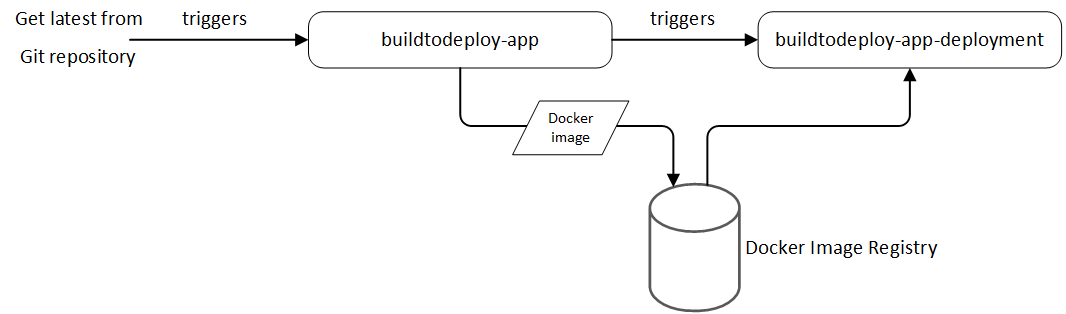
\includegraphics[width=\textwidth]{images/DockerPipeline.png}
	\caption{De pipeline van Docker containers\label{fig:cicd_pipeline}}
\end{figure}

\subsection{Git repository}
Eerst gaan we een Git repository maken met een test applicatie. De applicatie is een simpele rekenmachine met enkele JUnit-tests (Figure \ref{fig:calculator_app}).

\begin{figure}[H]
	\begin{center}
		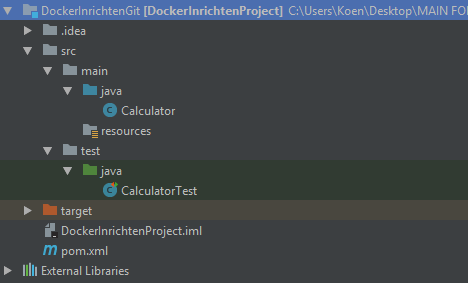
\includegraphics[width=0.75\textwidth]{images/CalculatorApplication.png}
		\caption{De structuur van de Calculator applicatie\label{fig:calculator_app}}
	\end{center}
\end{figure}

De Git repository heeft alleen een master branch. Dit is prima voor nu, maar in een echt project is het beter om het systeem van branches uit het releaseplan te gebruiken. Dat branch systeem is ingericht voor CI/CD gebruik.

\subsection{Jenkins container}
Nu gaan we een Docker container maken waar Jenkins op draait. Deze container moet zo worden ingericht dat Jenkins de Git repository weet te vinden, de tests gedraaid worden, en uiteindelijk een nieuwe Docker container aanroept.
\linebreak
In plaats van op een schone container Jenkins te installeren maken we gebruik van de kracht van Docker. Op de Docker Hub is een kant-en-klare Jenkins image te vinden. Deze kan gepulled worden met het volgende commando:

\begin{lstlisting}[language=Bash]
docker pull jenkins/jenkins
\end{lstlisting}

\noindent We kunnen de image openen met het volgende commando\textsuperscript{\cite{jenkins_documentation}}:

\begin{lstlisting}[language=Bash]
docker run -p 8080:8080 -p 50000:50000 -v jenkins_home:/var/jenkins_home jenkins/jenkins:latest
\end{lstlisting}

\noindent De docker instance draait, en heeft poort 8080 gemapped, zoals we hadden meegegeven in het commando. Nu moeten we Jenkins configureren. Hiervoor moet een wachtwoord ingevoerd worden, welke te vinden is in de console window.

Eerst moeten we aangeven waar de git repository staat:

\begin{figure}[H]
	\begin{center}
		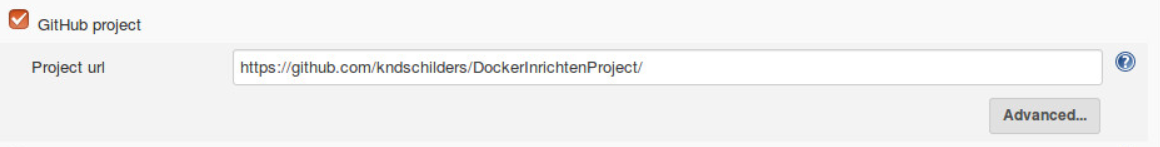
\includegraphics[width=1.0\textwidth]{images/Jenkins-Github.PNG}
		\caption{GitHub repository instellen\label{fig:jenkins_config_repo}}
	\end{center}
\end{figure}

\noindent Jenkins heeft user credentials nodig, en moet weten van welke branch hij de applicatie moeten halen.

\begin{figure}[H]
	\begin{center}
		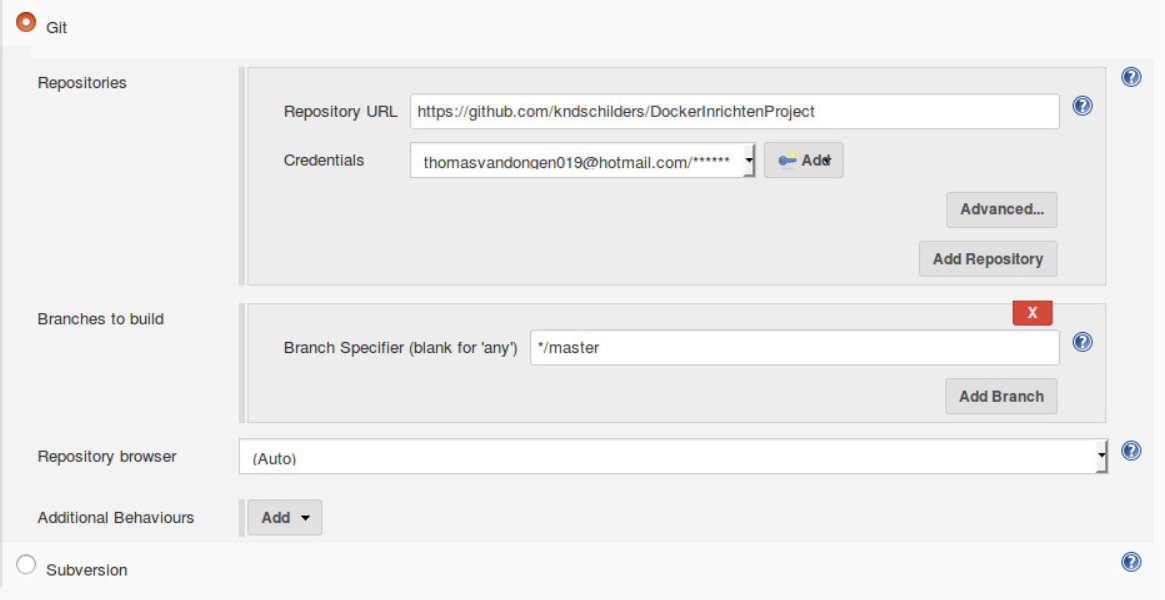
\includegraphics[width=1.0\textwidth]{images/Jenkins-Github-2.PNG}
		\caption{GitHub instellen\label{fig:jenkins_config_repo_2}}
	\end{center}
\end{figure}

\noindent Met Maven kan de applicatie gebuild worden. Uiteraard moet er eerst gecleaned worden (want het is Java). Hierna kan er gebuild en getest worden.

\begin{figure}[H]
	\begin{center}
		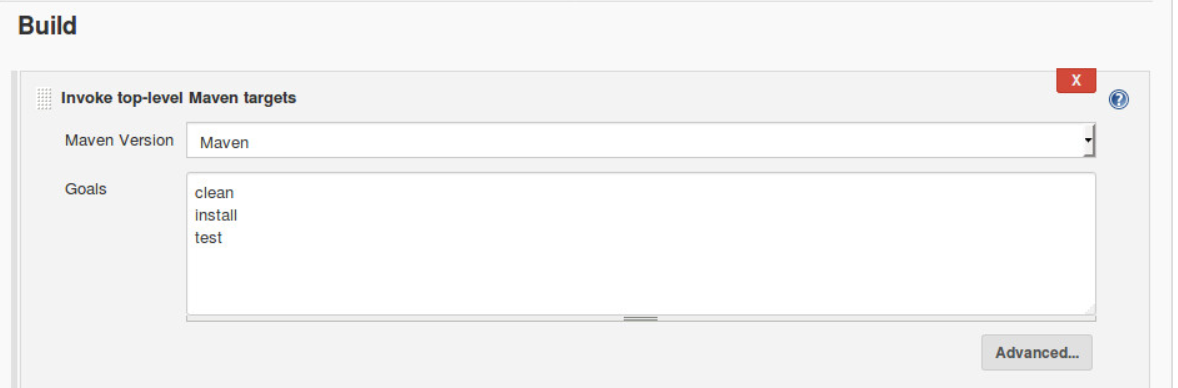
\includegraphics[width=1.0\textwidth]{images/Maven.PNG}
		\caption{Maven instellen\label{fig:jenkins_maven}}
	\end{center}
\end{figure}

\noindent Als laatste moeten er mail notifications ingesteld worden. Hier wordt simpelweg een email-adres ingevoerd. Als Jenkins iets te melden heeft wordt er naar dit email-adres een mailtje verstuurd.

\begin{figure}[H]
	\begin{center}
		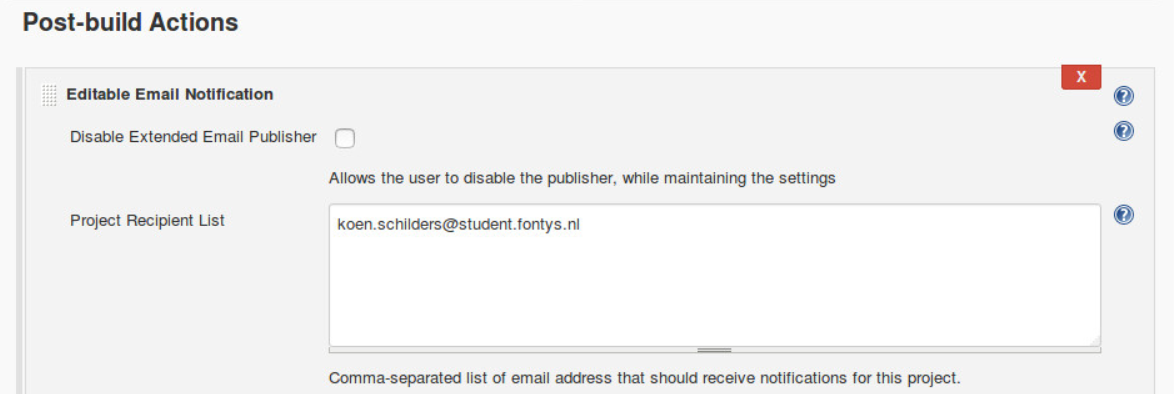
\includegraphics[width=1.0\textwidth]{images/Postbuildaction.PNG}
		\caption{Email notifications instellen\label{fig:jenkins_config_email_notifications}}
	\end{center}
\end{figure}

\noindent Jenkins is nu correct geconfigureerd.

\subsection{Deployment container}
\noindent De Jenkins container is klaar, en de image (een war-file) wordt in de shared volume folder gezet. Nu moet de .war file draaien in een andere container.

We hebben gekozen om de war-file in een Glassfish container te draaien. We pullen eerst een Glassfish image: 

\begin{lstlisting}[language=Bash]
docker oracle/glassfish:latest
\end{lstlisting}

\noindent Er moet een Glassfish container gemaakt worden, welke gebaseert is op de Glassfish image. Deze container moet toegang krijgen tot de war file gemaakt door de Jenkins container, omdat deze war gepubliseert gaat worden. Daarnaast moeten de IP's gemapped worden zodat we de gepubliseerde applicatie kunnen bereiken vanaf het host systeem. Dit kan allemaal in één run-commando:

\begin{lstlisting}[language=Bash]
docker run -i -t -p 4848:4848 -p 8181:8181 -v "/var/lib/docker/volumes/jenkins_home/_data/workspace/SOP6 Docker/target":/glassfish5/glassfish/domains/domain1/autodeploy oracle/glassfish:latest
\end{lstlisting}

\begin{figure}[H]
	\begin{center}
		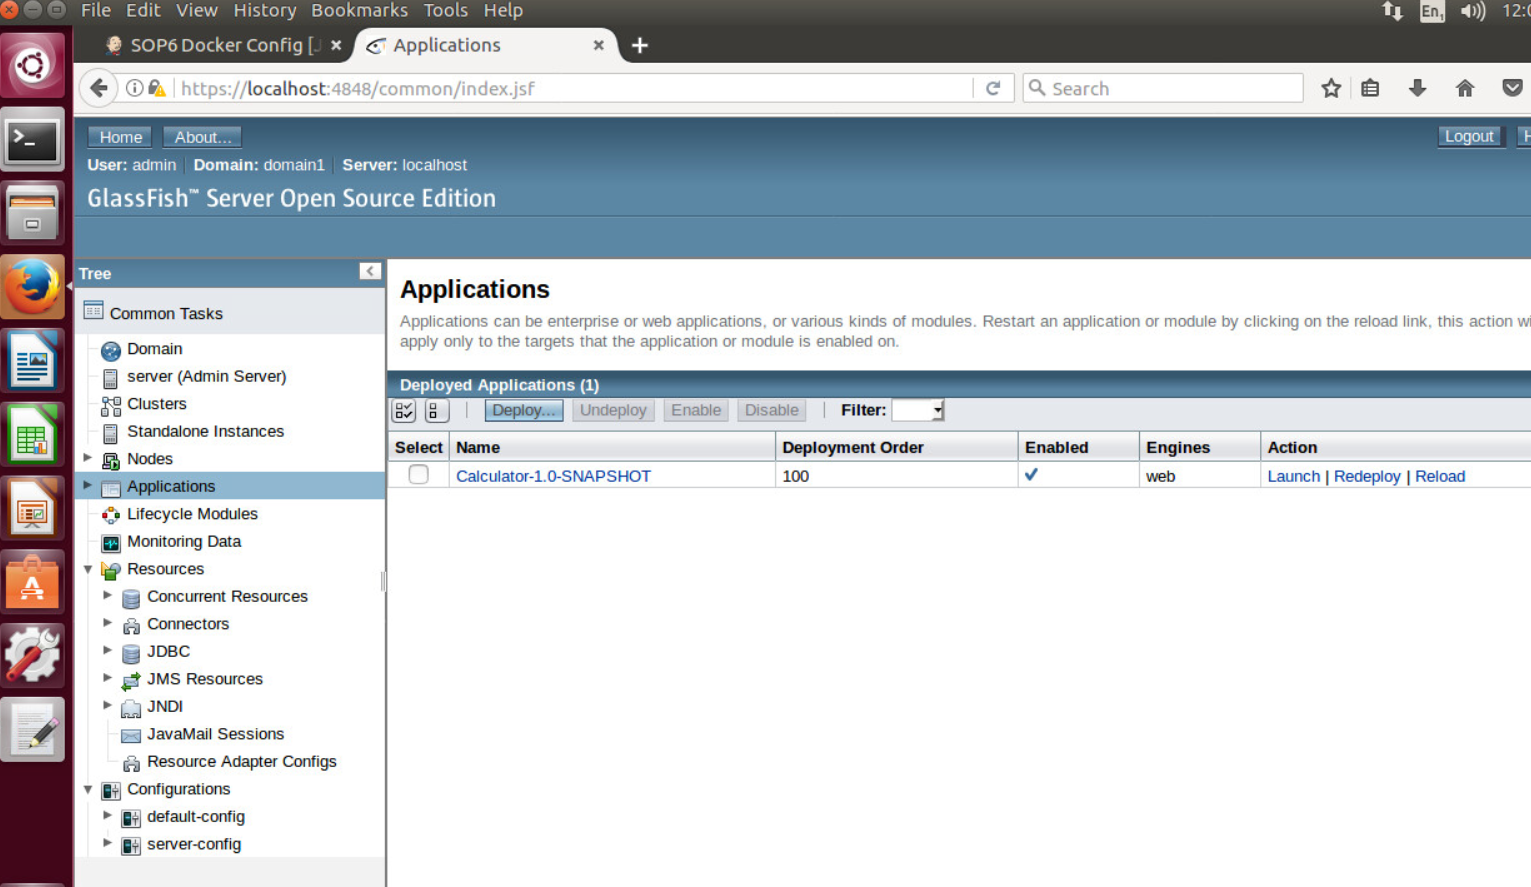
\includegraphics[width=1.0\textwidth]{images/applications_glassfish.png}
		\caption{Glassfish heeft de war gevonden\label{fig:glassfish_application}}
	\end{center}
\end{figure}

\noindent Met dit commando wordt een nieuwe Glassfish container aangemaakt. De IP's en volumes zijn gemapped.

% Sources
\begin{thebibliography}{9}
	\bibitem{jenkins_documentation}
		Tom Hipkin,
		\textit{Official Jenkins Docker image},
		24 januari 2018,
		\url{https://github.com/jenkinsci/docker/blob/master/README.md}
\end{thebibliography}
\end{document}